\section{Evoluzione stellare}\linkdest{stellarevolution}

\begin{wordonframe}{da fare: kippenhahn wiegert}
\begin{itemize}
\item main sequence 207'-214' (110-114)
\item Hayashi line 224'-232' (119-123)
\item Stability 234'-246 (124-130)
\item Onset of star formation 248'-255' (131-134)
\item Formation of protostars 256'-265' (135-139)
\item pre-main sequence contraction 266'-270' (140-142)
\item from initial to present sun 271'-276' (142-144)
\item chemical evolution in MS 277'-291' (145-152)
\item He-burning: massive stars 292'-307' (153-160)
\item He-burning:low-mass stars 308'-327' (161-170)
\item Later phases:  328'-343' (171-178)
\item Explosion and collapse 344'-364' (179-189)
\end{itemize}
\end{wordonframe}

\begin{frame}[allowframebreaks]{List of things}
%\printbibliography[keyword={inference},heading=beamer]
%\printbibliography[keyword={\mybibcat},heading=beamer]
\listofkeywords
\end{frame}

\subsection{Pre main sequence ed approccio a ZAMS per stelle di sequenza superiori/inferiori}\linkdest{preMS}

\begin{frame}{Traccia di Hayashi}
Primo/secondo core di Larson; Evoluzione di PMS sulla traccia di Hayashi; ruolo di opacit\'a di H- nella verticalit\'a della traccia di Hayashi; fusione deuterio; stelle completamente convettive o con nucleo radiativo. Abbondanza elementi leggeri in stelle di pre-sequenza
\end{frame}

\begin{frame}{Approccio alla ZAMS per stelle di sequenza superiori/inferiori}
dipendenza della ZAMS dall'abbondanza originale di He e metalli; metodo determinazione $DY/DZ$ dal confronto teoria-osservazione per stelle di disco locale parallassate; dipendenza massa minima di transizione dall'abbondanza di He e metalli; influenza sulla ZAMS dell'incertezza degli input fisici e dell'efficienza della convezione
\end{frame}

\subsection{Evoluzione di sequenza principale}\linkdest{MS}

\begin{frame}{Yield of H-burning star analysis}
\begin{itemize}
\item Longest evolutionary phase: larger number of observed stars
\item central/shell-H-burning determine successive phases
\item most important clock is central H-burning termination
\item Final shell H-burning phase in low mass, low-Z star provide distance indicator for old stellar pop
\item count of stars evolving through central H-burning give insight on IMF
\end{itemize}
\end{frame}

\begin{frame}{Major H burning reaction: PP chains}
\begin{columns}[T]\begin{column}{0.45\textwidth}
\begin{align*}
&T\leq\SI{5e6}{\kelvin}\\
&^1H+^1H\to^2D+\APelectron+\Pnue\\
&^2D+^1H\to^3He+\gamma\\
&T\geq\SI{8e6}{\kelvin}:\\
&^3He+^3He\to^4He+2^1H\tag*{PPI}\\
&T\geq\SI{15e6}{\kelvin}:\\
&^3He+^4He\to^7Be+\gamma\\
&^7Be+\Pelectron\to^7Li+\Pnue\\
&^7Li+^1H\to^4He+^4He\tag*{PPII}\\
&^7Be+^1H\to^8B+\gamma\\
&^8B\to^8Be+\APelectron+\gamma\\
&^8Be\to2^4He
\end{align*}
\end{column}\begin{column}{0.55\textwidth}
\begin{align*}
&r_{pp}=\num{11.5e10}\rho^2X_H^2T_6\expy{-2/3}\\
&\exp{-33.81T_6\expy{-1/3}}(1+\num{0.0123}T_6\expy{1/3}+\num{0.0109}T_6\expy{2/3}\\
&+\num{0.00095}T_6)\\
&\rho\epsilon(3H\to^3He)=\\
&(\SI{6.936}{\mega\ev}-\SI{0.263}{\mega\ev})*\SI{1.602e-6}{\erg}*r_{pp}\\
&\rho\epsilon(^3He(^3He,2p)^4He)=\\
&(\SI{6.936}{\mega\ev}-\SI{0.263}{\mega\ev})*\SI{1.602e-6}{\erg}*r_{pp}\\
&\frac{PPI}{PPII+PPIII}=\frac{r_{33}}{r_{34}}=\frac{\lambda_{33}(^3He)^2/2}{\lambda_{34}^3He^4He}
\end{align*}
\end{column}\end{columns}
\end{frame}

\begin{frame}{H burning: CN-NO cycle}
\begin{columns}[T]\begin{column}{0.5\textwidth}
Ciclo CN-NO
\begin{align*}
&^{12}C+^1H\to^{13}N+\gamma\\
&^{13}N\to^{13}C\APelectron+\Pnue\\
&^{13}C+^1H\to^{14}N+\gamma\\
&^{14}N+^1H\to^{15}O+\gamma\\
&^{15}O\to^{15}N+\APelectron+\Pnue\\
&^{15}+^1H\to^{12}+^4He\tag*{CN}\\
&T\geq\SI{20e6}{\kelvin}\tag*{\num{e-4} volte}\\
&^{15}N+^1H\to^{16}O+\gamma\\
&^{16}O+^1H\to^{17}F+\gamma\\
&^{17}F\to^{17}O+\APelectron+\Pnue\\
&^{17}O+^1H\to^{14}N+^4He
\end{align*}
\end{column}\begin{column}{0.5\textwidth}
\begin{align*}
&\epsilon_{CN}(T_6)=\epsilon_{CN}(25)(\frac{T_6}{25})^{16.7}
\end{align*}
\end{column}\end{columns}
\end{frame}

\subsection{Lower main sequence ($M^*\leq1.3\msun{}$)}\linkdest{LMS}

\begin{frame}{Da ZAMS a TO for $M^*\leq1.3\msun{}$}
ZAMS: first MS model fully supported by H-burning in which secondary elements are in equilibrium:
\begin{itemize}
\item $^3He$ production in central zones: si forma piccolo core convettivo
\[\TDy{t}{N_3}=N_1N_2\exv{\sigma v}_{12}-2\frac{(N_3)^2}{2}\exv{\sigma v}_{33}-N_3N_4\exv{\sigma v}_{34}\]
\end{itemize}
\begin{columns}[T]\begin{column}{0.4\textwidth}
\begin{figure}[!ht]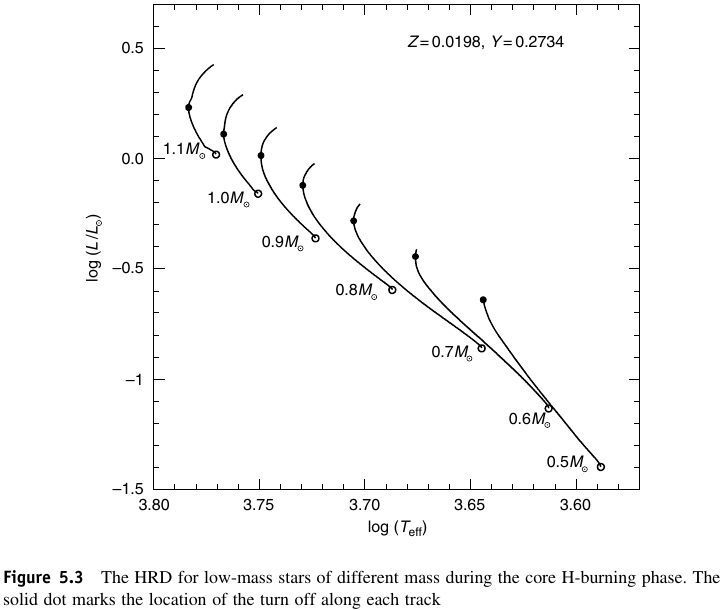
\includegraphics[trim={0cm 0cm 0 0},clip, keepaspectratio,width=0.99\textwidth]{HRD-LMS}\label{fig:HRD-LMS}
\end{figure}
\end{column}\begin{column}{0.6\textwidth}
La stella continua a contrarsi fino alla partenza della reazione $^3He(^3He,2^1H)^4He$ e il core convettivo svanisce con l'espandersi della regione in cui \'e prodotto $^3He$
Struttura: H-burn in central radiative core (Small T-dep of $\epsilon_{PP}$), convective core (large opacity associated to partial ionized H, He)
Evoluzione: $\#$ free particles $\downarrow$, \xaumenta{\mu} per HE \xaumenta{T}
, \xdiminuisce{R} quindi $L^*$ aumenta lentamente.
TO is hottest point in evolutionary track: H exhausted 
\end{column}\end{columns}
\end{frame}


\subsection{Upper main sequence ($M^*\geq1.2-1.3\msun{}$)}\linkdest{UMS}

\begin{frame}{Da ZAMS a Overall contraction}
\begin{columns}[T]\begin{column}{0.4\textwidth}
\begin{figure}[!ht]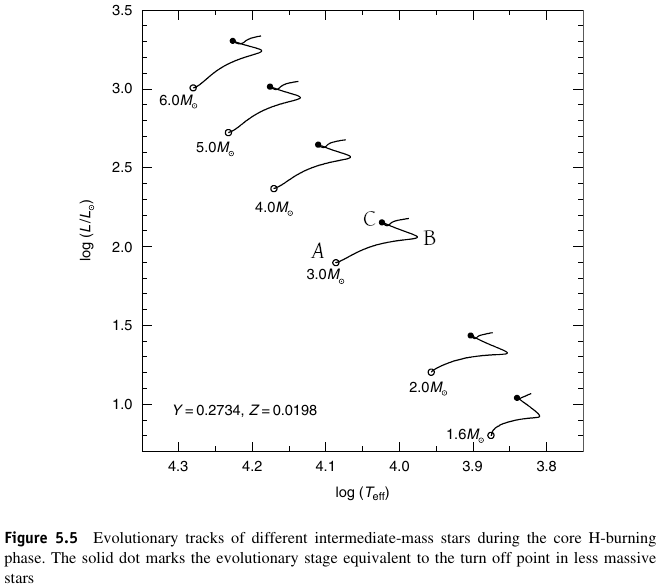
\includegraphics[trim={0cm 0cm 0 0},clip, keepaspectratio,width=0.99\textwidth]{HRD-UMS}\label{fig:HRD-UMS}
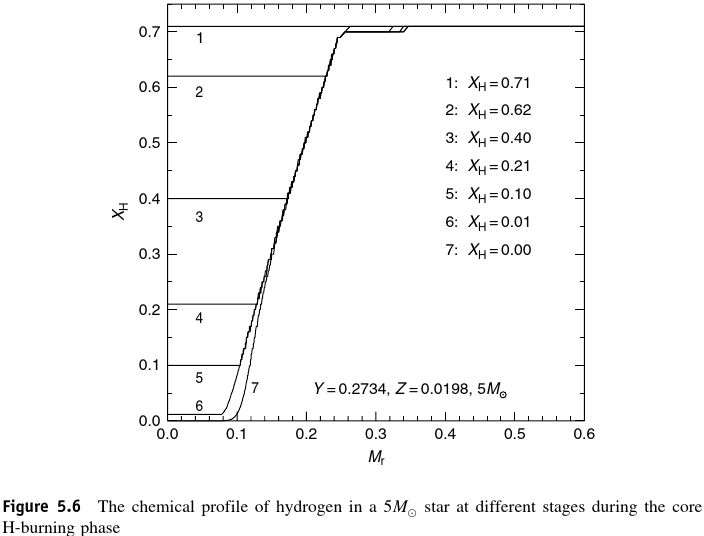
\includegraphics[trim={0cm 0cm 0 0},clip, keepaspectratio,height=0.42\textheight]{UMS-Hprofile}\label{fig:UMS-Hprofile}\end{figure}
\end{column}\begin{column}{0.6\textwidth}
\begin{block}{CNO H-Burning: convective core}
Higher T: CNO dominant: $\epsilon_{CNO}$ steeper:convective core: \xaumenta{M^*}, \xaumenta{M_{con}}, \xaumenta{P_{rad}}, \xdiminuisce{\nad{}}.
\end{block}
\begin{block}{As UMS burn H}
\begin{itemize}
    \item convective core shrink: ?\xaumenta{\mu}, \xaumenta{P_c}?
    \item radius expands: after H exhaustion
    \item core gravitationally contract
    \item $L$ increases such that $T_e$ has little drop
\end{itemize}
\end{block}
\begin{block}{Overall contraction}
When $X<0.05$ at B start gravitational contraction of core until C; after C inner regions contract outer expand
\end{block}
\end{column}\end{columns}
\end{frame}

\subsection{Deps of MS on Physical input}

\begin{frame}{Effects of changes in initial chemical composition}
\begin{block}{Different initial Y value: opacity and mean molecular weight}
\begin{columns}[T]
\begin{column}{0.5\textwidth}
\begin{figure}[!ht]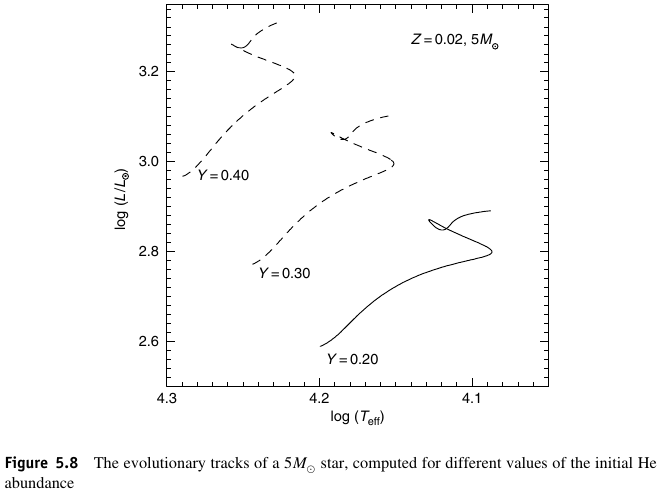
\includegraphics[trim={0cm 0cm 0 0},clip, keepaspectratio,width=0.99\textwidth]{HRD-changingHe}\label{fig:HRD-changingHe}
\end{figure}
\end{column}
\begin{column}{0.5\textwidth}
\begin{itemize}
    \item Increases of nuclear rates $L_H\propto\mu^7$
    \item Opacity decreases
\end{itemize}
Star is brighter and hotter
\end{column}
\end{columns}
\end{block}
\begin{block}{Changes in Z affect opacity}
\begin{itemize}
    \item \xaumenta{Z}, \xaumenta{\kappa}: fainter, cooler star.
    \item PP chain reaction not dependent on Z, CNO element are enough exept in pop III.
    \item $\alpha$-enhanced objects: CNO cycle efficiency increased, opacity increased with two bump at $\log{T}=6,5.5$ due to K shell O electrons and L-edges of Mg, Si, Ne. Stars are fainter and cooler
\end{itemize}
\end{block}
\end{frame}

\begin{frame}{Effects of changing convection efficiency: superadiabatic convection}
\begin{columns}[T]
\begin{column}{0.5\textwidth}
\begin{figure}[!ht]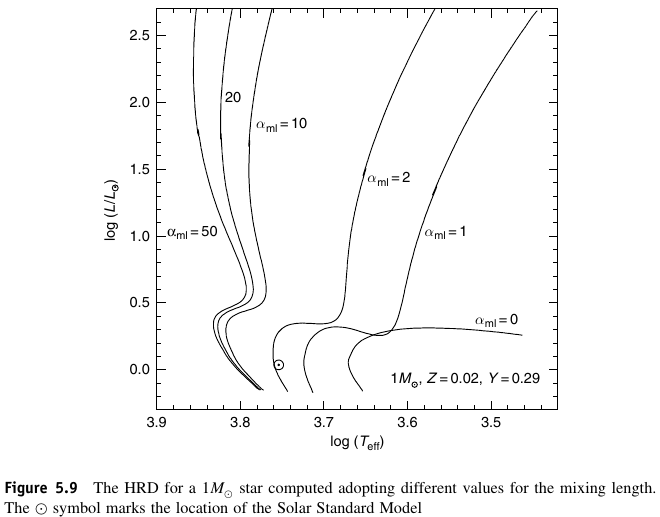
\includegraphics[trim={0cm 0cm 0 0},clip, keepaspectratio,width=0.99\textwidth]{HRD-1M-changingalpha}\label{fig:HRD-changingHe}
\end{figure}
\end{column}
\begin{column}{0.5\textwidth}
\begin{itemize}
    \item $\alpha_{ML}$ calibrated using Sun.
    \item $\alpha_{ML}$ does not affect L
    \item $\alpha_{ML}$ radius and $T_e$: \xaumenta{\alpha},\xdiminuisce{\nabla},\xaumenta{T_e},\xdiminuisce{R_s}
\end{itemize}
\end{column}
\end{columns}
\end{frame}

\begin{frame}{Convective core and Overshooting ($M>10\msun{}$)}
\begin{columns}[T]\begin{column}{0.5\textwidth}
\begin{figure}[!ht]
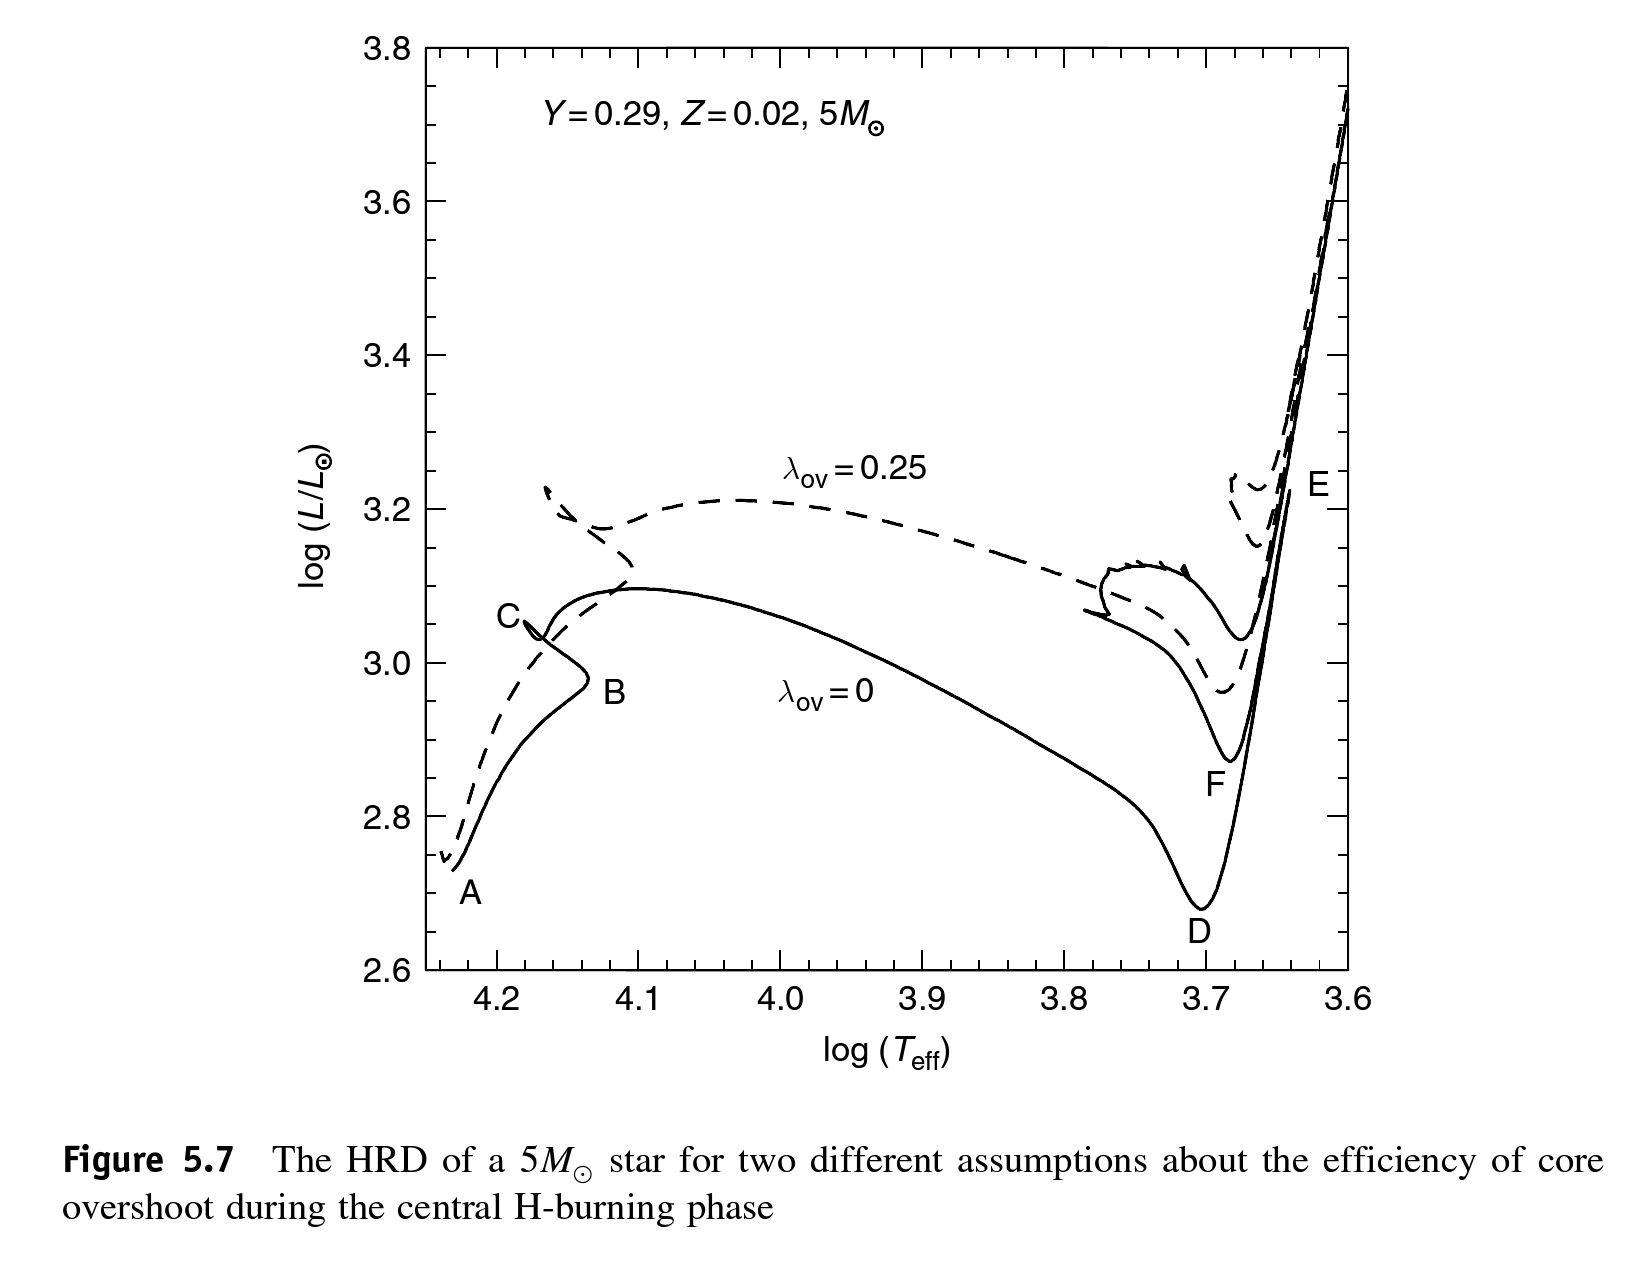
\includegraphics[trim={0cm 0cm 0 0},clip, keepaspectratio,height=0.42\textheight]{HRD-overshoot}\label{fig:HRD-overshoot}
\end{figure}
\end{column}
\begin{column}{0.5\textwidth}
\begin{block}{What increases convective core}
\begin{itemize}
\item Changes in physical input
\item Stellar rotation
\item Physical overshooting
\end{itemize}
\end{block}
\end{column}\end{columns}
\begin{columns}[T]\begin{column}{0.55\textwidth}
\begin{block}{Effects of increased convective core}
\begin{itemize}
\item \xaumenta{M_c}, \xaumenta{\mu} (involve more mass), \xaumenta{L}
\item Longer central H-burning
\item Larger He core at end of MS: brighter He-burning phase star, shorted lifetime
\end{itemize}
\end{block}
\end{column}
\begin{column}{0.45\textwidth}
\begin{block}{\sch vs Ledoux in-stability criterion}
In radiative region the retracting convective core leave chem composition gradient; but \xaumenta{He}, \xdiminuisce{\kappa}
\end{block}
\end{column}\end{columns}
\end{frame}

\begin{frame}{Low-mass star $M<0.4\msun{}$}
\begin{columns}[T]\begin{column}{0.4\textwidth}
\begin{figure}[!ht]
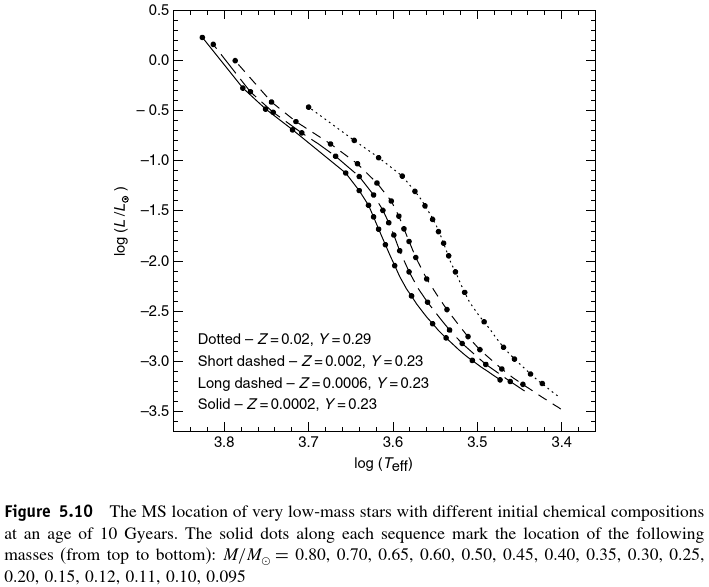
\includegraphics[trim={0cm 0cm 0 0},clip, keepaspectratio,width=0.99\textwidth]{VLM-HDR}\label{fig:VLM-HDR}
\end{figure}
\end{column}
\begin{column}{0.6\textwidth}
\begin{itemize}
    \item Fully convective through MS live
    \item PP1 H-burning with negligible $^3He$ destruction
    \item Transition between molecular H and atomic He to plasma at inner $90\%$ in mass: thermodynamical properties sensible to treatment of pressure ionizzation, dissociation, non-ideal Coulomb.
    \item Atmospheric features due to opacity sources: collisional induced dipole in $H_2$ molecules, CIA suppresses flux at \SI{2}{\micro\meter}; for $T_e<\SI{4000}{\kelvin}$ molecules of $TiO$ and $VO$ controll flux in optical, $H_2O$ and $CO$ the flux in infrared; for $T_e<\SI{2800}{\kelvin}$ also grains are important.
\end{itemize}
\end{column}\end{columns}
\end{frame}

\subsection{Mass-Luminosity relations}

\begin{frame}{M-L relation}
Near ZAMS $L\propto M^3$. Assumption: radiative transport $L\propto\frac{R^4}{M}T^4$, HE $P\propto M^2/R^4$, perfect gas $P\propto\rho T$.
\begin{columns}[T]\begin{column}{0.5\textwidth}
\begin{figure}[!ht]
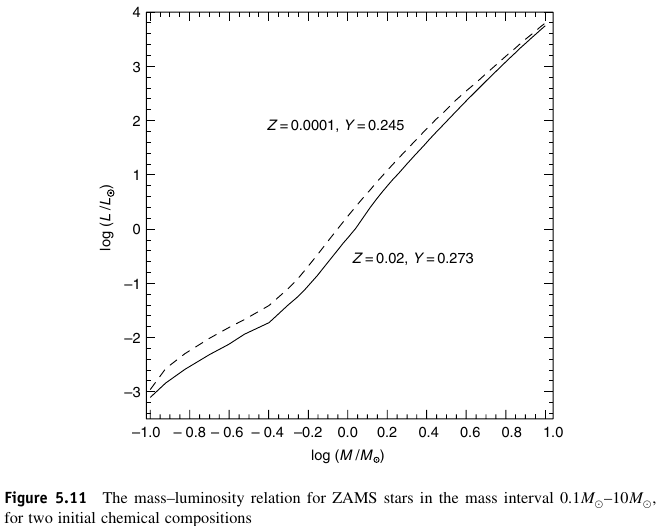
\includegraphics[trim={0cm 0cm 0 0},clip, keepaspectratio,width=0.99\textwidth]{ML-01-10}\label{fig:ML-01-10}
\end{figure}
\end{column}
\begin{column}{0.5\textwidth}
Relazione osservativa
\begin{equation*}
L\propto\begin{array}{l}
M,\ M>10\msun{}\\
M\expy{3.6},\ \numrange{2}{20}\msun{}\\
M\expy{4.5},\ \numrange{0.5}{2}\msun{}\\
M\expy{2.6},\ \numrange{0.2}{0.5}\msun{}\\
\end{array}
\end{equation*}
\end{column}\end{columns}
\end{frame}

\subsection{Post-MS}
%SC [160]

\begin{frame}{Condizione Core per fusione}
\begin{figure}[!ht]
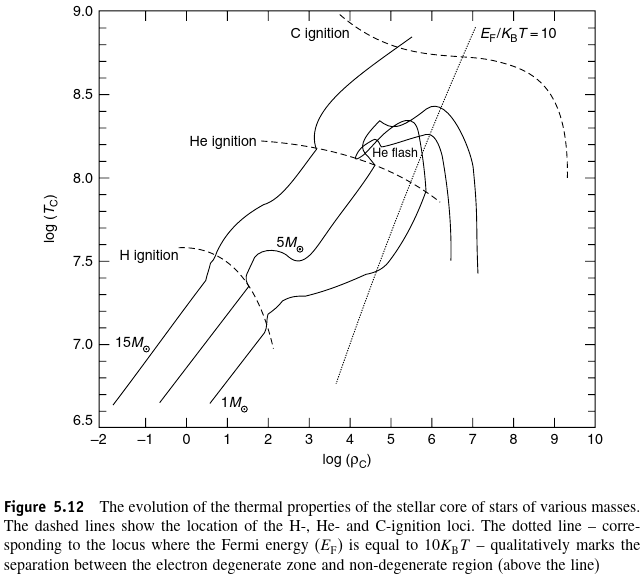
\includegraphics[trim={0cm 0cm 0 0},clip, keepaspectratio,height=0.4\textheight]{HHeCcore}\label{fig:HHeCcore}
\end{figure}
\begin{itemize}
    \item Electron degeneracy
    \item gravitational contraction: virial theorem
\end{itemize}
\end{frame}

\begin{frame}{SC-mass limit}
$L=0$ implica formazione core di He isotermo: se la massa del core di elio \'e maggiore del $10\%$ della massa totale della stella il core si contrae - le stelle della LMS hanno core pi\'u piccolo, stelle di massa $M\geq2.5-3\msun{}$  hanno core pi\'u grande.
\begin{equation*}
\frac{M_c}{M}>(\frac{M_c}{M})_{SC}=0.37(\frac{\mu_{env}}{\mu_c})^2\xrightarrow{\parbox{2.5cm}{$\mu_e=\mu_{\odot}=0.6$\\$\mu_c=\mu(He)=1.3$}}0.08
\end{equation*}
il core si contrae su $\tkh{}$.
Virial theorem for non-vanishing pressure surface pressure $P_0$ and $M_c$, $R_c$ and $T_c$:
\begin{align*}
&(2U_i+\Omega+S_p=0,\ S_p=-\int\exv{v^2}\Vec{r}\cdot\hat{n}\,dS=P_0V)\\
&P_0=K_1\frac{M_cT_c}{R_c^3}-K_2\frac{M_c^2}{R_c^4}\\
&P_{0,m}=K_3T_c^4/M_c^2
\end{align*}
For equilibrium $P_{0,m}\geq P_e\propto M_t^2/R^4=T_c^4/M_t^2$ ($T_c\propto M_t/R$)
\end{frame}

\begin{frame}{Int-massive stars: from SG to RG}
\begin{columns}[T]\begin{column}{0.44\textwidth}
\begin{figure}[!ht]
%trim: LBRT
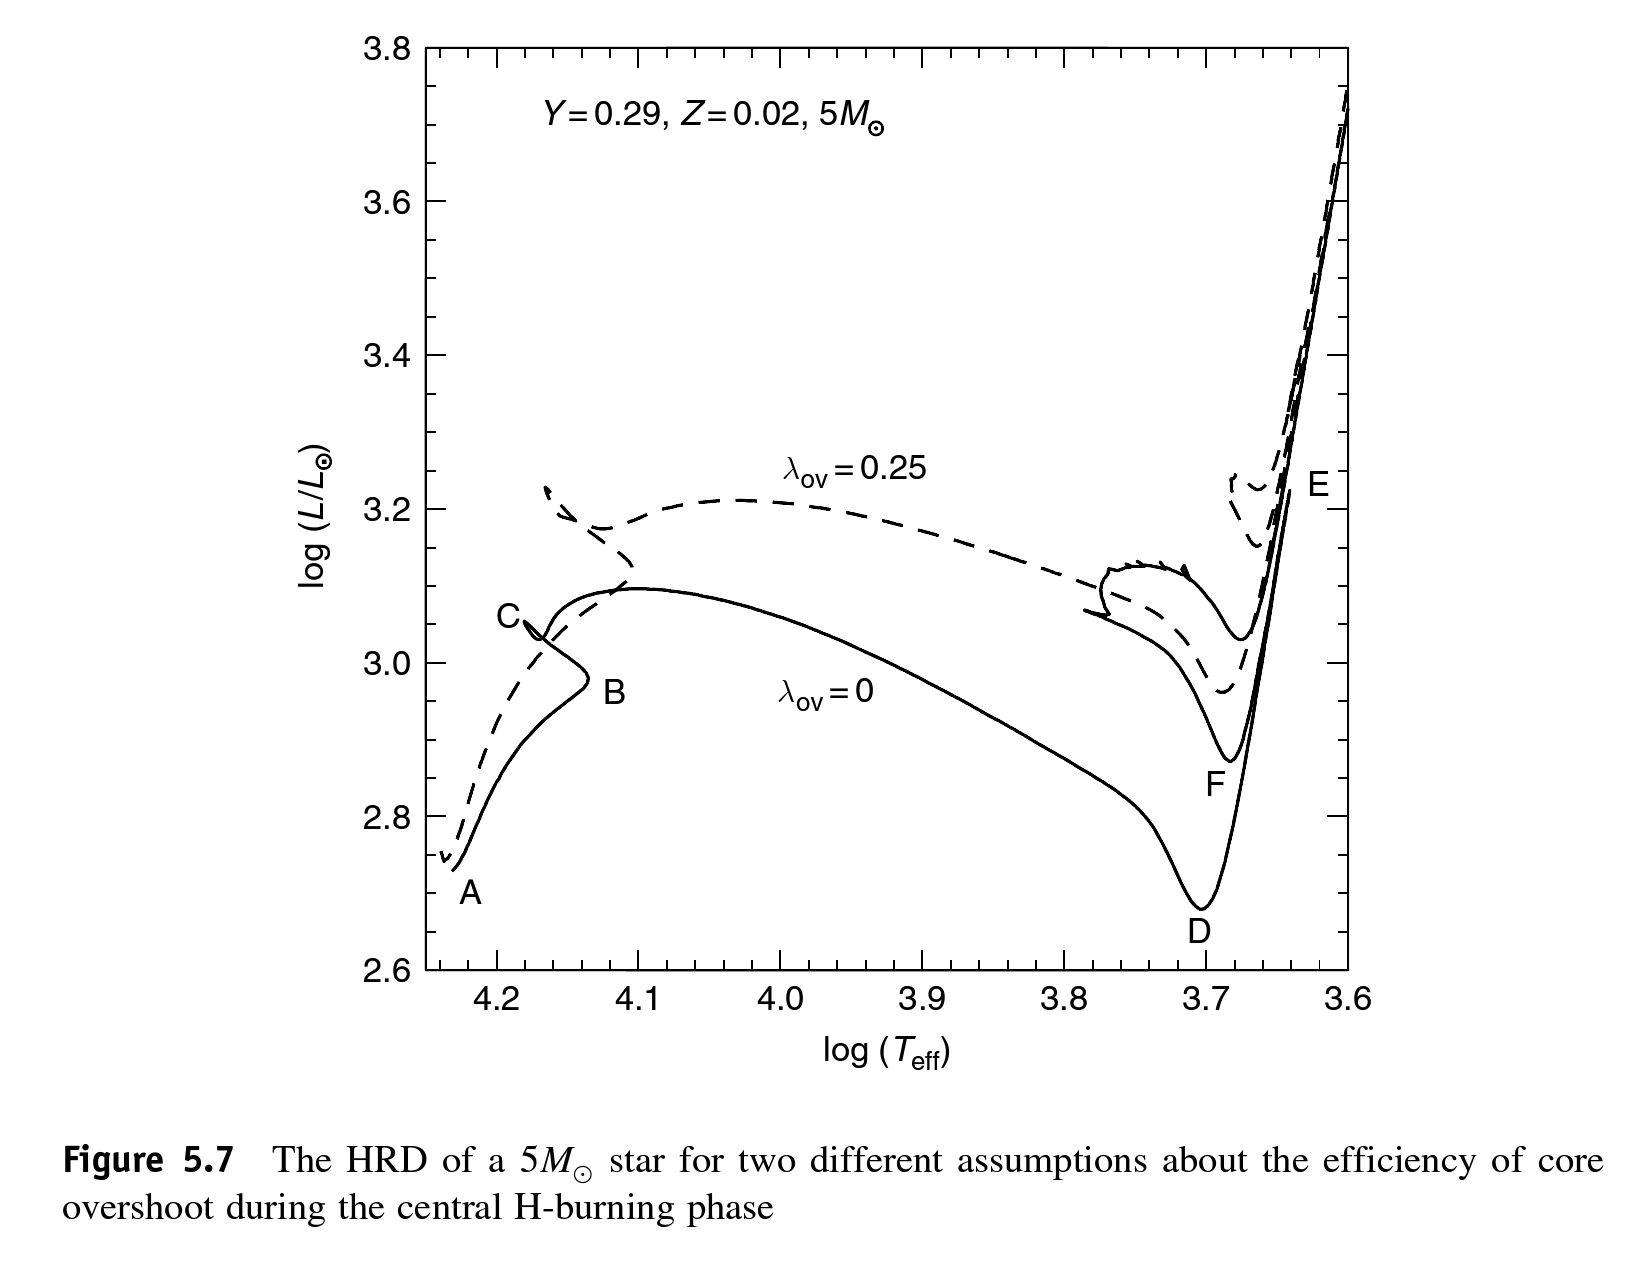
\includegraphics[trim={2cm 2cm 3cm 1cm},clip, keepaspectratio,width=0.99\textwidth]{HRD-overshoot}\label{fig:HRD-overshoot}
\end{figure}
\end{column}
\begin{column}{0.55\textwidth}
\begin{itemize}
    \item $M_c>M_{SC}$ ($M\approx2.3-3$ dopo H-burning in shell): He core contract
    \item broad shell of CNO H-burning: $\epsilon_g$ changes sign at max $\epsilon_{CNO}$ - envelope expand: \xdiminuisce{T_e}, \xaumenta{\kappa_e} quindi inviluppo diventa convettivo.
    \item Star move from B to R at constant L - Hertzsprung gap: $\begin{array}{c}\tkh{}(3\msun{})\approx\SI{12}{\mega\year}\\\tkh{}(6\msun{})\approx\SI{1}{\mega\year}\end{array}$
\end{itemize}
\end{column}\end{columns}
\begin{itemize}
    \item In (D) star reaches Hayashi track where begins RG phase: $T_e$ costante, \xaumenta{L}
    \item $\rho_c$ suff. low such onset of \Pelectron degeneracy is avoided: in (E) contracting core reaches $T\approx\SI{e8}{\kelvin}$ for efficient He-burning. \xaumenta{M_c} (VT: \xaumenta{T_c}) \xdiminuisce{\tau_{RG}}
\end{itemize}
\end{frame}

%trim: LBRT
\begin{frame}{Low-mass stars}
\begin{columns}[T]\begin{column}{0.44\textwidth}
\begin{figure}[!ht]
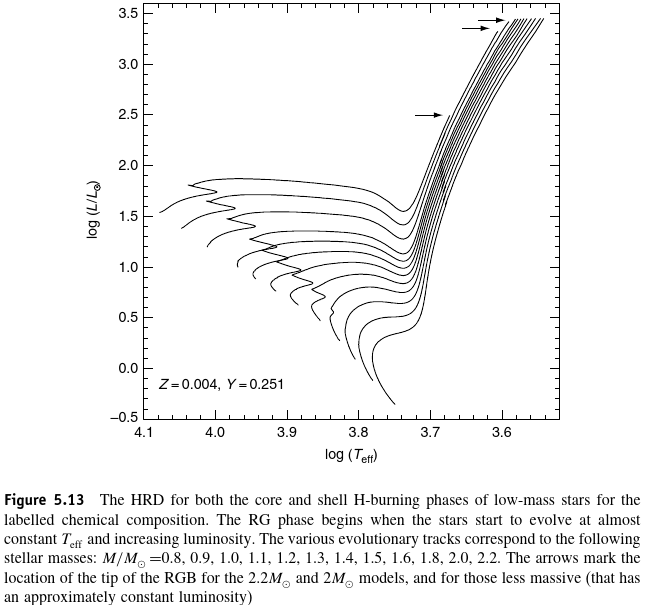
\includegraphics[trim={0cm 0cm 0cm 0cm},clip, keepaspectratio,width=0.99\textwidth]{HDRtipRGB}\label{fig:HDRtipRGB}
\end{figure}
\end{column}
\begin{column}{0.55\textwidth}
\begin{itemize}
\item As X exhausts max $\epsilon_H$ is no more in central region (at TO at $M_r=0.1\msun{}$). He Core (radiative/small convective??): $M<M_{SC}$, high electron degeneracy.
\item From TO to RG H-burning shell becomes thinner due to CNO deps on T that decreses in envelop and to X exhaustion.
\end{itemize}
\end{column}\end{columns}
\begin{itemize}
\item $M_{cHe}-L$ relation: \xaumenta{M_{cHe}}, \xaumenta{L}. L is almost fully provided by H-burning shell whose thermal properties are determined $R_c$, $M_c$ ($P_e$ is OM lower)
\item RGB stars evolve at constant L and radius re-adjust to stellar mass: mass loss shift $T_e$ toward lower values.
\end{itemize}
\end{frame}

\begin{frame}{Envelop structure: depth of convection and first dredge-up}
\begin{columns}[T]\begin{column}{0.44\textwidth}
%trim: LBRT
\begin{figure}[!ht]
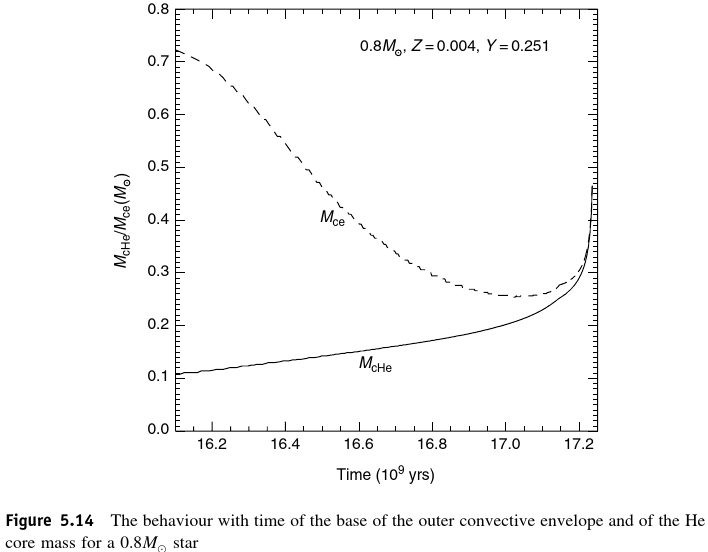
\includegraphics[trim={0cm 0cm 1cm 0cm},clip, keepaspectratio,height=0.35\textheight]{postMS-depthC}\label{fig:postMS-depthC}
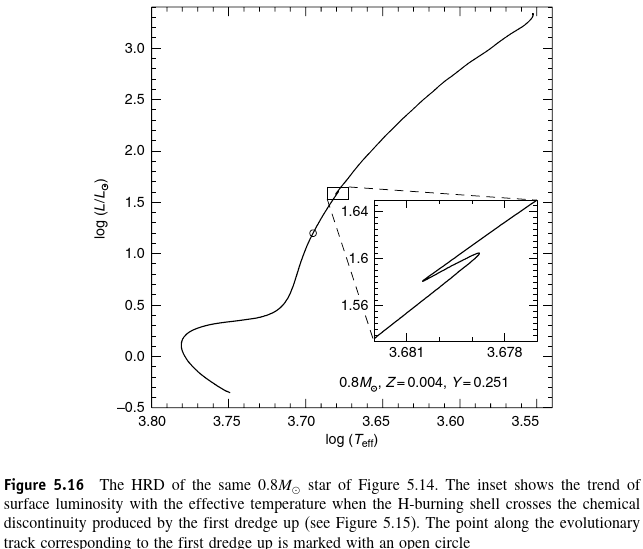
\includegraphics[trim={0cm 0cm 1cm 0cm},clip, keepaspectratio,height=0.35\textheight]{HburnxIdu}\label{fig:HburnxIdu}
\end{figure}
\end{column}
\begin{column}{0.55\textwidth}
\begin{itemize}
\item Cooling of envelop causes deeper convection that reaches a maximum before RG (\xdiminuisce{T}, \xaumenta{\kappa}). Primo dredge-up: \xaumenta{He_s}, \xaumenta{^{14}N_s}, \xdiminuisce{^{12}C} ($\frac{^{12}C}{^{13}C}$), $Li$, $Be$ reduces several OM.
\item In RGB phase H-burning shell move outward and convective zone move toward surface: chemical discontinuity at max convective depth. \keyword{Bump of RGB}: as H-burning shell meet discontinuity $L_H\propto\mu^7$ diminish the in fully mixed envelop \xaumenta{L} as \xaumenta{M_{cHe}} - bump in RGB luminosity function ($20\%$ rgb-time in this luminosity range)
\end{itemize}
\end{column}\end{columns}
\end{frame}

\begin{frame}{\keyword{Thermal runaway at tip of RGB}: He-flashes}
\begin{columns}[T]\begin{column}{0.44\textwidth}
%trim: LBRT
\begin{figure}[!ht]
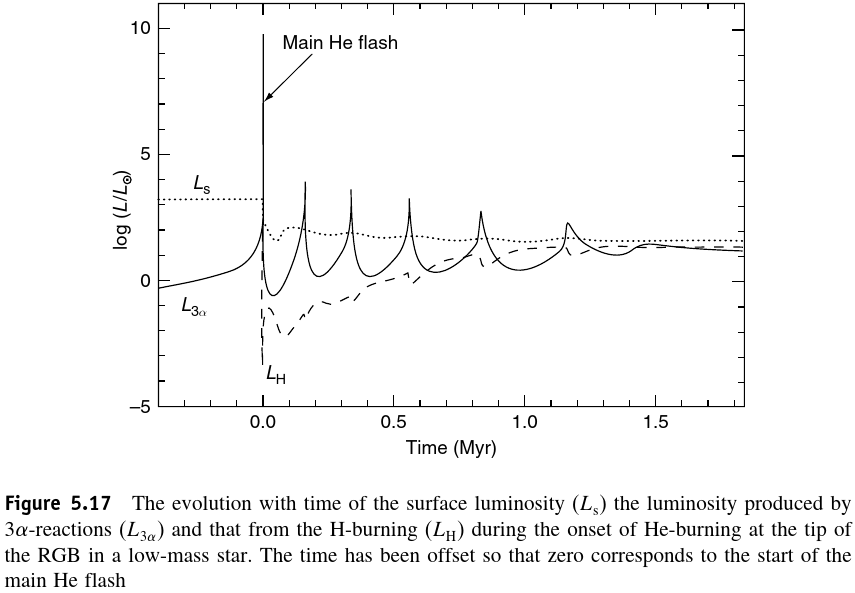
\includegraphics[trim={0cm 0cm 1cm 0cm},clip, keepaspectratio,width=0.99\textwidth]{He-flash}\label{fig:He-flash}
\end{figure}
\end{column}
\begin{column}{0.55\textwidth}
In RG phase: H-burning increases $M_{cHe}$ and \xaumenta{\rho_c}. In inner part $M_r<0.3M_t$ when $\epsilon_g+\epsilon_{\nu}<0$: $\TDy{r}{L}<0$ resulting in T-inversion. \xaumenta{\rho_c}, grado di degenerazione aumenta, \xdiminuisce{\kappa_{cond}}, \xdiminuisce{T_c}; while \xaumenta{T_c^M} due to $\epsilon_g>0$ at boundary between D/ND matter. At $T_c^M\approx\SI{e8}{\kelvin}$ we have He ignition ($M_{cHe}\approx0.48-0.5\msun{}$): end of RGB phase.
\end{column}\end{columns}
He ignition at strong partial-relativistic-D ($\rho_x\approx\SI{e6}{\gram\per\cubic\cm}$, $T\approx\SI{8e7}{\kelvin}$), $P$ is insensitive to $T$ changes, rate of $3\alpha$-burning increases much: thermal runaway $\num{e10}\lsun{}$ in few seconds are absorbed by above ND layers: expansion and convection (large jump in P/S prevent mixing with above H-burning). So \xaumenta{T} at constant $\rho$ but no time for heat diffuse the whole core: this need many successive He-flashes, $\tau_{flash}\approx\SI{e6}{\year}$ and $5\%$ He converted to C
\end{frame}

\begin{wordonframe}{SC: WD cooling $[22], [45]$, Z poor $[196]$}

\end{wordonframe}

\subsection{Deps of RGB on params}

\begin{frame}{Location of RGB on HRD}
\begin{itemize}
\item Highly Z-dependent: size of convective envelop (Hayashy track) \xaumenta{Z}, \xaumenta{\kappa}, inviluppo convettivo pi\'u grande:  $\alpha$-enhanced stars (more low ionization potential: Mg, Si, ...) form molecule $TiO$ and $H^-$: RGB cooler and less steeper.
\item \xaumenta{Y}, \xdiminuisce{\kappa}, \xdiminuisce{CE}, \xaumenta{T_e}
\item RGB is important Z indicator of galaxies/star clusters
\item $\rho_e$ low: $\nabla_e$ \'e super-adiabatico (\xaumenta{
\alpha_{ML}},\xaumenta{T_e})
\item \keyword{RGB phase transition}. \xdiminuisce{M_*}, \xdiminuisce{T_e}: $M_{cHe}$ constant for $M\leq1.8\msun{}$ then decreases with $M$ as degeneracy is completely removed 
\end{itemize}
\end{frame}

\begin{frame}{Deps RGB's L-bump on params}
\begin{columns}[T]\begin{column}{0.55\textwidth}
%trim: LBRT
\begin{figure}[!ht]
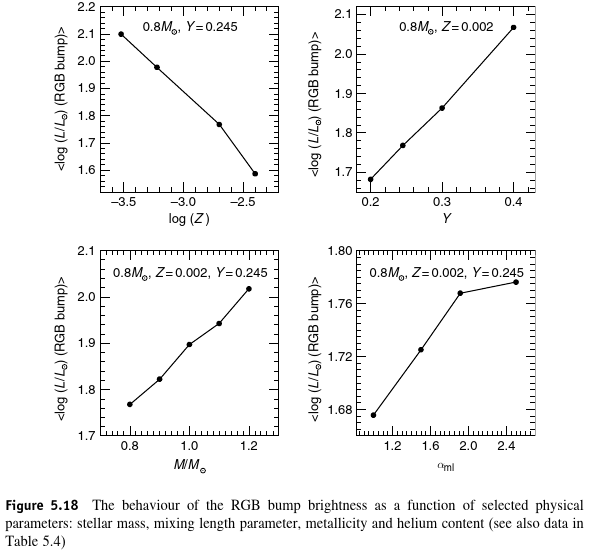
\includegraphics[trim={0cm 0cm 1cm 0cm},clip, keepaspectratio,width=0.99\textwidth]{RGB-bumpparams}\label{fig:RGB-bumpparams}
\end{figure}
\end{column}
\begin{column}{0.45\textwidth}
As convection zone goes deeper the H-burning shell takes less time to cross chemical discontinuity: (\xdiminuisce{M_*}/\xaumenta{Z}/\xdiminuisce{Y},\xdiminuisce{\alpha_{ML}}), \xdiminuisce{L_{bump}}
\end{column}\end{columns}
\end{frame}

\begin{frame}{Deps RGB tip's (He-ignition) luminosity on params}
\begin{columns}[T]\begin{column}{0.44\textwidth}
%trim: LBRT
\begin{figure}[!ht]
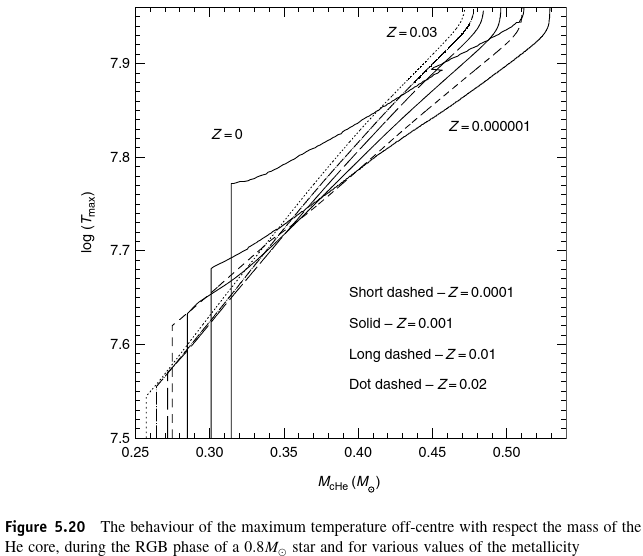
\includegraphics[trim={0cm 0cm 1cm 0cm},clip, keepaspectratio,height=0.36\textheight]{RGBTmax}\label{fig:RGBTmax}
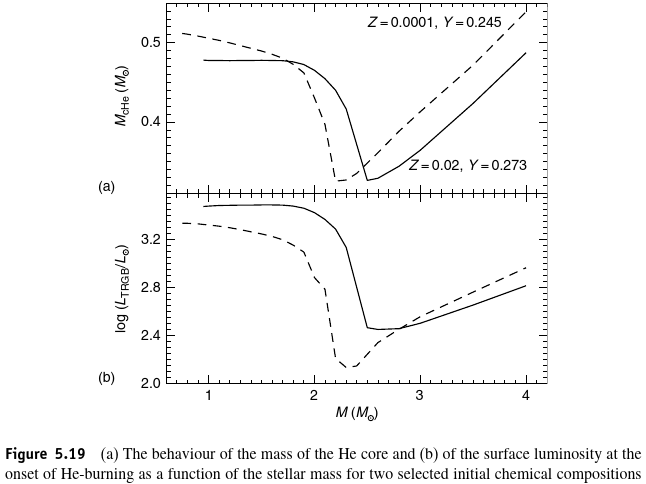
\includegraphics[trim={0cm 0cm 1cm 0cm},clip, keepaspectratio,height=0.36\textheight]{HecLsatHeburning}\label{fig:HecLsatHeburning}
\end{figure}
\end{column}
\begin{column}{0.55\textwidth}
\begin{itemize}
    \item \keyword{RGB phase transition}. \xdiminuisce{M_*}, \xdiminuisce{T_e}: $M_{cHe}$ constant for $M\leq1.8\msun{}$ then decreases with $M$ as degeneracy is completely removed then increases as consequences of larger convective H-burning core.
    \item \xaumenta{He}, \xaumenta{T_c}, deg \Pelectron diminuisce, $M_{cHe}$ He-ignition diminuisce, \xdiminuisce{L_{TIP}}
    \item \xaumenta{Z}, \xaumenta{\epsilon_{CNO}}, $M_{cHe}$-ignition is builded faster since He production is faster and He-core heating is faster, \xaumenta{L_{TIP}}
\end{itemize}
\end{column}\end{columns}
\end{frame}

\subsection{Very low Z stars}

\begin{frame}{Very low Z (pop III)}
\begin{itemize}
    \item Primordial star (Pop III) responsable for Z-enrichment: from $Z\approx\numrange{e-10}{e-12}$ to $Z\approx\numrange{e-2}{e-3}$ (Pop II)
    \item High mass star burn H through PP chain so need much higher T; as $T\approx\SI{e8}{\kelvin}$ He-burning produce $^{12}C$: threshold for CNO H-burning to begins $X_C\approx\numrange{e-9}{e-10}$
    \item \xaumenta{M_*}, \xdiminuisce{\tau_{PP\to CNO}}: transition to convective core for $M>2\msun{}$ (for $M=2-5\msun{}$ convective core after $^3He$ production phase).
    \item RGB phase transition at lower mass/higher age: for low mass star \xaumenta{T_c}, degenerazione elettronica del core di He diminuisce, faster He ignition, \xdiminuisce{M_{cHe}}, \xdiminuisce{L_{TIP}}
    \item Intermediate mass star have no RGB
\end{itemize}
\end{frame}

\subsection{Combustione He in nucleo di He non degenere}\linkdest{ZAHB}

\begin{frame}{Memo per HB}
combustion di He per stelle medio-grandi; clump He; loop He; Esaurimento He centrale: , semiconvezione e pulsi convettivi
\end{frame}

\begin{frame}{ZAHB: equilibrium model and nuclear reaction sunto}
\begin{columns}[T]
\begin{column}{0.45\textwidth}
\begin{block}{equilibrium model}
\begin{itemize}
\item $\tau_{He-Flash}\approx\SI{e6}{\year}$: after that time of He-burning the \Pelectron degeneracy is removed (small obser. prob). Some authors start He-core evolution sequence from C enriched equilibrium model
\item \keyword{ZAHB}: model where He is burnt into chem homo-core and H in shell with chem stratification He-flash like
\item He-enriched by I dredge-up
\item Rotation (dalayed He-flash): \xaumenta{M_{cHe}}, \xdiminuisce{M_*} (mass loss), \xaumenta{T^{ZAHB}}/\xaumenta{L^{ZAHB}}
%\xaumenta{\epsilon_{He}}/\xdiminuisce{\epsilon_H}
\end{itemize}
\end{block}
\end{column}
\begin{column}{0.55\textwidth}
\begin{block}{He-burning reactions}
\begin{align*}
&3\alpha (T\gtrsim\SI{1.2e8}{\kelvin}):\\ &^4He+^4He\to^8Be\tag*{$\tau_{1/2}\approx\SI{e-16}{\second}$}\\
&^8Be+^4He\to^{12}C+\gamma\tag*{$\SI{7.27}{\mega\ev}$, $\tau_H\approx100\tau_{He}$}\\
&\epsilon_{3\alpha}\approx\begin{array}{c}T^{40}: T\approx\SI{e8}{\kelvin}\\T^{20}: T\approx\SI{2e8}{\kelvin}\end{array}\\
&^{12}C+\alpha\to^{16}O+\gamma\\
&^{16}O+\alpha\to^{20}Ne+\gamma\\
&^{20}Ne+\alpha\to^{24}Mg+\gamma\\
&^{24}Mg+\alpha\to^{28}Si+\gamma
\end{align*}
\end{block}
\end{column}
\end{columns}
\end{frame}

\begin{frame}{ZAHB in HDR}
	contenu...
\end{frame}

\begin{frame}{ZAHB dep on core (and envelope) mass}
\begin{itemize}
\item Structure and evolution of ZAHB fixed by: $M_*$, $M_{cHe}$ (for $M<1.8\msun{}$ $t_{TIP}>4-5\si{\giga\year}$: $M_c$ weakly dependent on M), $Y$, $Z_e$ - For fixed composition, $L_s$ is fixed by $M_{cHe}$ (then by $M_e$): important standard candles for Pop II stars (\keyword{Standard candles: HB brightness}). $(\TDy{M_{cHe}}{\log{L_{ZAHB}^{\log{T_e}=3.85}}})_{Y,Z}\approx3.04$
\item Location in HDR: \xdiminuisce{M_e}, \xaumenta{T_e} - HB (slightly oblique due to \xaumenta{\epsilon_H},\xaumenta{M_e}). $T_e\approx\SIrange{3500}{4000}{\kelvin}$ for $M_e\approx\numrange{e-4}{0.4}\msun{}$ (RGB mass loss)
\item \xaumenta{R_{cHe}}, \xdiminuisce{L_s} from RGB-tip as H-burning shell cool down
\item He-burning in convective core (steep T deps)
\item H-burning in shell: for fixed $M_{cHe}$ efficiency determined by \xaumenta{M_e}, \xaumenta{\epsilon_H}
\end{itemize}
\end{frame}

\begin{frame}{ZAHB dep on composition}
\begin{columns}[T]
\begin{column}{0.55\textwidth}
\begin{itemize}
\item \xaumenta{Y_{in}}, \xdiminuisce{M_{cHe}}, \xaumenta{L_H}/\xdiminuisce{L_{cHe}}, $L^{ZAHB}$ approx const: B part of ZAHB becomes fainter/ R part brighter. $(\TDy{Y}{L_{ZAHB}^{3.85}})_{M_{cHe},Z}\approx2.07$
\item \xaumenta{Z_{in}}, \xdiminuisce{M_{cHe}^{Flash}}/\xaumenta{\kappa_e}, \xdiminuisce{L^{ZAHB}}/\xdiminuisce{T_e^{ZAHB}}. $(\TDy{Z}{L_{ZAHB}^{3.85}})_{M_{cHe},Y}\approx-0.04$
\end{itemize}
\end{column}
\begin{column}{0.45\textwidth}
\begin{figure}[!ht]
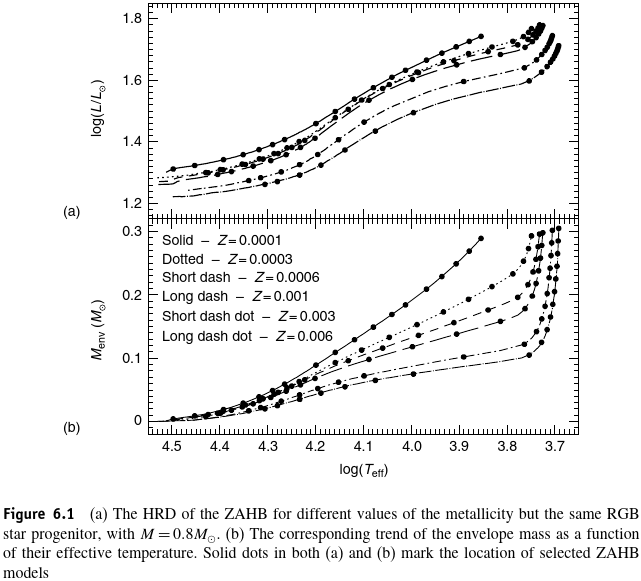
\includegraphics[trim={0cm 0cm 1cm 0cm},clip, keepaspectratio,height=0.37\textheight]{HDR-ZAHB-M08}\label{fig:HDR-ZAHB-M08}
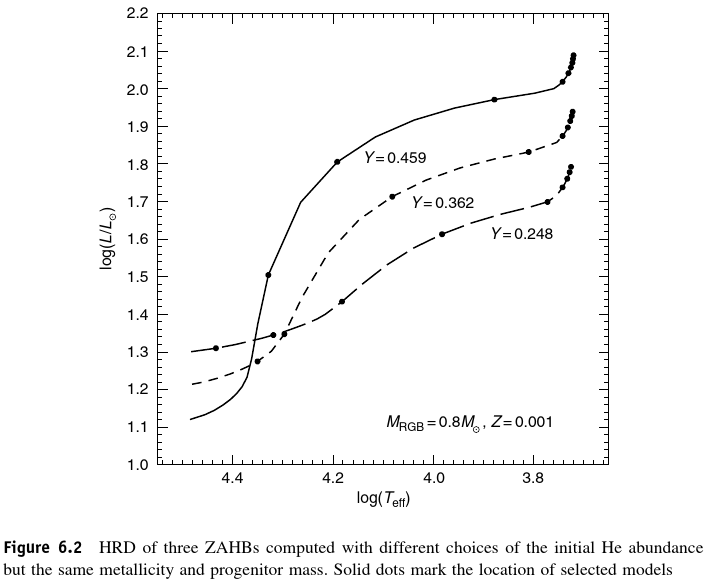
\includegraphics[trim={0cm 0cm 1cm 0cm},clip, keepaspectratio,height=0.37\textheight]{HDRZAHBdiffY}\label{fig:HDRZAHBdiffY}
\end{figure}
\end{column}
\end{columns}
\end{frame}

\subsection{Core He-burning in low-mass stars}

\begin{frame}{HB evolution in HDR}
\begin{columns}[T]
\begin{column}{0.5\textwidth}
\begin{itemize}
\item \xaumenta{\epsilon_{He}}, \xdiminuisce{\epsilon_H}: as $L_{He}<L_H$ star evolves at \xaumenta{T_e}, $L_{He}>L_H$ star moves toward R. (Loop)
\end{itemize}
\end{column}
\begin{column}{0.5\textwidth}
\begin{figure}[!ht]
%\includegraphics[trim={0cm 0cm 1cm 0cm},clip, keepaspectratio,height=0.37\textheight]{ffiig}\label{fig:ffiigg}
\end{figure}
\end{column}
\end{columns}
\end{frame}

\begin{frame}{Mixing processes and physical properties evolution}
\begin{columns}[T]
	\begin{column}{0.5\textwidth}
\begin{block}{Convective instability}
Mixing processes in convective He-burning core: $\tau_{con}\ll\tau_{nuc}$, as $^4He\to^{12}C$, \xaumenta{\kappa_{ff}} ($\propto X_iZ_i^2$), \xaumenta{\nrad{}} - growing discontinuity in T gradient at convective core boundary - overshoot cause mixing with radiative shell: \xaumenta{\kappa} - convective instability of boundary - selfdriving mechanism for extension of convective core - Convective boundary is established where $\nabla_{ad}=\nabla_{rad}$
\end{block}
\begin{block}{semi-convection}
$\nrad{}$ show a minimum due to outward shift in He-rich environment (complex behaviour of $\nrad$ due to local L, T, $\kappa$, P) - physical/chemical coupling convective zone outside minimum and mass of surrounding radiative layers - mixing of radiative shell: \xdiminuisce{\nad{}} in convective envelope (He-rich matter/properties of mixed shell) - convective core/convective shell not fully mixed: extended partially mixed semi-convection zone outside convective core between $\nrad$ minimum and radiative region
\end{block}
 	\end{column}
	\begin{column}{0.5\textwidth}
		\begin{figure}[!ht]
			%\includegraphics[trim={0cm 0cm 1cm 0cm},clip, keepaspectratio,height=0.37\textheight]{ffiig}\label{fig:ffiigg}
		\end{figure}
	\end{column}
\end{columns}
\end{frame}

\begin{frame}{Discussioni parametri che influenzano HB}
Parametro R per determinazione He
\end{frame}

\subsection{Core He-burning in Int/Mas stars}


\subsection{Ramo asintotico (AGB)}

\begin{frame}{Evoluzione in AGB}
Ingresso in agb: clump. AGB manqu\'e. Secondo Dredge-up; pulsi termici; terzo dredge-up
\end{frame}

\begin{frame}{Nucleosintesi in AGB}
Elementi s:tasca C13. Produzione di Li
\end{frame}

\subsection{Destino finale di stelle massicce}

\begin{frame}{Destino finale di stelle di varia massa}
nane bianche di He, C/O, O/Ne; supernovae di tipo II da deflagrazione del carbonio e cattura elettronica su nuclei; supernovae di tipo II da fotodisintegrazione del ferro; Caratteristiche di pre-SN; Neutronizzazione esplosiva e esplosione ritardata; classificazione SN in base a spettro e morfologia curva di luce
\end{frame}

\begin{frame}{Caratterizzazione SNII}
$Fe60$ come indicatore esplosioni nelle vicinanze della terra negli ultimi milioni di anni; Interazione neutrini-nucleo denso: intrappolamento e tempi scala emissione; stima energia emessa: neutrini, fotoni, fronte di shock; SN1987A: flusso di neutrini e osservazione in bande EM
\end{frame}


\begin{frame}{Evoluzione di nane bianche}

\end{frame}

\subsection{Modello Solare standar}

\begin{frame}{Caratteristiche e metodo di calcolo}
eliosismologia e neutrini
\end{frame}

\subsection{Stelle pulsanti}

\begin{frame}{Striscia di instabilit\'a e tipi di stelle pulsanti}
RR LyrAE: diagramma di Bailey, curve di luce; relazioni periodo-luminosit\'a, massa-temperatura effettiva.
Parametro A come indicatore di He.
Stelle cefeidi; dicotomia di Oosterhoff
\end{frame}